\documentclass{article}\usepackage[]{graphicx}\usepackage[]{color}
%% maxwidth is the original width if it is less than linewidth
%% otherwise use linewidth (to make sure the graphics do not exceed the margin)
\makeatletter
\def\maxwidth{ %
  \ifdim\Gin@nat@width>\linewidth
    \linewidth
  \else
    \Gin@nat@width
  \fi
}
\makeatother

\definecolor{fgcolor}{rgb}{0.345, 0.345, 0.345}
\newcommand{\hlnum}[1]{\textcolor[rgb]{0.686,0.059,0.569}{#1}}%
\newcommand{\hlstr}[1]{\textcolor[rgb]{0.192,0.494,0.8}{#1}}%
\newcommand{\hlcom}[1]{\textcolor[rgb]{0.678,0.584,0.686}{\textit{#1}}}%
\newcommand{\hlopt}[1]{\textcolor[rgb]{0,0,0}{#1}}%
\newcommand{\hlstd}[1]{\textcolor[rgb]{0.345,0.345,0.345}{#1}}%
\newcommand{\hlkwa}[1]{\textcolor[rgb]{0.161,0.373,0.58}{\textbf{#1}}}%
\newcommand{\hlkwb}[1]{\textcolor[rgb]{0.69,0.353,0.396}{#1}}%
\newcommand{\hlkwc}[1]{\textcolor[rgb]{0.333,0.667,0.333}{#1}}%
\newcommand{\hlkwd}[1]{\textcolor[rgb]{0.737,0.353,0.396}{\textbf{#1}}}%
\let\hlipl\hlkwb

\usepackage{framed}
\makeatletter
\newenvironment{kframe}{%
 \def\at@end@of@kframe{}%
 \ifinner\ifhmode%
  \def\at@end@of@kframe{\end{minipage}}%
  \begin{minipage}{\columnwidth}%
 \fi\fi%
 \def\FrameCommand##1{\hskip\@totalleftmargin \hskip-\fboxsep
 \colorbox{shadecolor}{##1}\hskip-\fboxsep
     % There is no \\@totalrightmargin, so:
     \hskip-\linewidth \hskip-\@totalleftmargin \hskip\columnwidth}%
 \MakeFramed {\advance\hsize-\width
   \@totalleftmargin\z@ \linewidth\hsize
   \@setminipage}}%
 {\par\unskip\endMakeFramed%
 \at@end@of@kframe}
\makeatother

\definecolor{shadecolor}{rgb}{.97, .97, .97}
\definecolor{messagecolor}{rgb}{0, 0, 0}
\definecolor{warningcolor}{rgb}{1, 0, 1}
\definecolor{errorcolor}{rgb}{1, 0, 0}
\newenvironment{knitrout}{}{} % an empty environment to be redefined in TeX

\usepackage{alltt}
% \usepackage{showframe} % uncomment to show margins
\usepackage{hyperref}

\title{Creating a Team Agreement}
\author{Marc Los Huertos}
%\date{} % Uncomment to remove date from document
%\date{09/01/2016} % Uncomment to create a specified date

\newcommand*{\SignatureAndDate}[1]{%
  \par\noindent\makebox[2.5in]{\hrulefill} \hfill\makebox[1.2in]{\hrulefill}%
  \par\noindent\makebox[2.5in][l]{#1}      \hfill\makebox[1.2in][l]{Date}%
}%
\IfFileExists{upquote.sty}{\usepackage{upquote}}{}
\begin{document}

\maketitle

\section{Introduction}

Building an effective team is not an automatic process. It requires time and effort. This handout is meant to facilitate the create and development of effective teams.\footnote{This document is new to my courses, so please feel free to submit suggestions to improve it.}

For this activity, you will explore what encourages good team work and how you might be participating in postive team. Once your team discusses each section, your team create your own team agreement (see template in Github/Admin), as a contract. After writing this contract, you will compile the PDF, print, and sign the document. Finally, once it has been signed by all parties, scan and upload this document to your team folder, so the document can facilitate project management.

\section{Reflections on Team Project Experiences}

Take 5 minutes to reflect on your experiences in projects that required work as a team by writing out responses to the following prompts:

\begin{itemize}
  \item Describe several positive and negative experiences.
  \item What things allowed negative characteristics of the experiences?
  \item What encouraged the success of the team work?
  \item What did you learn from these experiences?
\end{itemize}

As a group of team members, describe experiences that you have had working in teams. 

\subsection{Running List of Experiences}

\subsubsection{Negative Experiences}
\begin{itemize}
\item 1
\end{itemize}

\subsubsection{Positive Experiences}
\begin{itemize}
\item 1
\end{itemize}


\section{Some Conclusions on Effective Teams}

Below is a summary of conclusions based on research regarding what makes effective teams. Many of these are designed for corporate contexts, so they will require some translation for course-based projects.

Take a few minutes to read each of these outloud and discuss what these goals mean in our context.

\subsection{Focusing on Goals}

According to the research, a team is driven by a common goal. In order to have an effective team, that common goal is articualted in advance and understood by each team member. By focusing on these team goals, a team has a better chance of success. 

\paragraph{Strategy 1:} Put the goals in writing so everyone can see and understand what the objectives of the team are and help to work toward accomplishing them.

\subsection{Compensation--Rewards--Grading}

In many cases, a team works well when members understand how they will be compensated for their efforts. Usually it's best to come up with a compensation plan before assembling the team. When people have their compensation expectations laid out before they sign an agreement to join the team, compensation can be removed as an obstacle to effective teamwork. If all team members feel they are being compensated (graded) fairly that can help lead to high productivity.

\begin{figure}
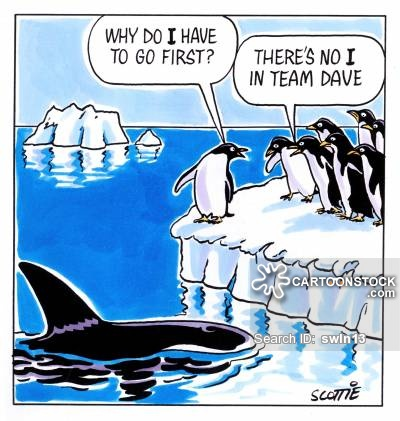
\includegraphics[width=.50\textwidth]{../../Graphics/PenguinTeamWork.jpg}
\caption{Working in a team is risky. How can we reduce the risk and increase the rewards?}
\end{figure}

On the other hand, some research has found the external motivators are only useful for physical activies and actually reduce performance in intellectually demanding activites. A good summary of this research can be found via the following website:

\url{https://www.youtube.com/watch?v=u6XAPnuFjJc&list=PL39BF9545D740ECFF&index=15}

We want to allow the following: 

\begin{itemize}
  \item Autonomy
  \item Mastery
  \item Challenge
  \item Purpose Driven
\end{itemize}

This line of thinking argues that the rewards are come from accolades, where creativity is an internal motivator, but that we should acknowledge that we want to be rewarded for our own work. So, based on this, for this course, grades, i.e. compensation, will be given based on individual work, where I can evaluate your contributution with more certainty than a group projects that hide individual contributions. 

\subsection{Communication}
Communication in developing an effective team happens on two levels: communication between team members and communication from management to the team. We should encourage open communication among team members, so they can learn how each other communicates. But does this gaurentee good communcation? Probably not!  Yet, we might still conclude that more communication is better than less. To facilitate this, we should have informal modes of communication as well as professional modes of communication. 

\paragraph{Strategy 2:} Encourage interaction between team members outside of the the classroom to develop better communication. 

In addition, the project managers plays a key role in the process. Managers should hold regular meetings to keep a team updated on important information and to provide resources to build skills. These are the kinds of tools a team needs from management to be effective. 

\paragraph{Strategy 3:} Project manager shall meet regularly with team members to ensure they have the resources needed and have developed good communication patterns.

\subsection{Deal With Conflict}

When working together, conflicts are bound to arise. We may have the perception that conflicts arise of some flaw, but they might come from difference in opinion or different values or different styles of interactions. None of these constitute an unusual circumstance or a failure of the group dynamic. However, serious conflicts can devastate a project's process. And even mild conflicts can influence how a group works together and the success of the public product. Conflict tends to throw a team off of its focus, getting it away from its goals and objectives. By learning to deal with conflict immediately, a team can remain effective at all times.

\paragraph{Strategy 4:} We will work together to address a conflict within a team as it arises. 

\begin{figure}
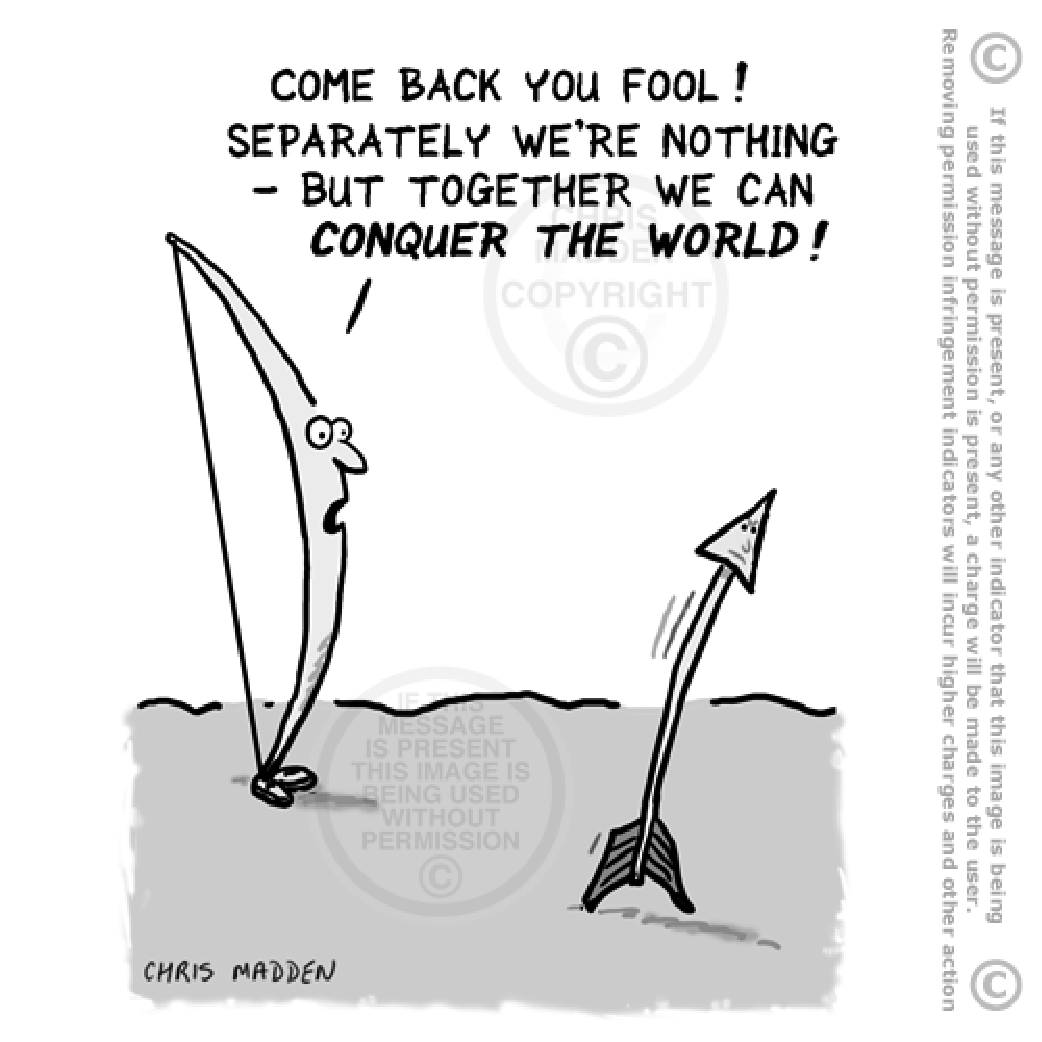
\includegraphics[width=.50\textwidth]{../../Graphics/Bow-arrow-conquer-world}
\caption{Resolving conflict is an art -- how we approach conflicts is key to the success of a team.}
\end{figure}

\section{Defining Goals for Team Work} 

After discussing the sections above, read over the following list of characteristics of good team work: 

\subsection{Unified Commitment to a Goal}
A team is created to complete the goals it is given. An effective team is committed to completing its goal by using the team's resources. It does not mean that as individuals the people that make up the team share the same point of view or are all in agreement on what is best for the group. It means that when the team is presented with a goal, they can come together and work as a single unit to complete the task.

\subsection{Participation}
For a team to act as a team everyone must be participating in the creation of a solution. A team does not have extra members. Each member of a team is essential to the team's success, and when the group is given a task, each member knows what their job is and sets out to put in their fair share of the effort.

\begin{figure}
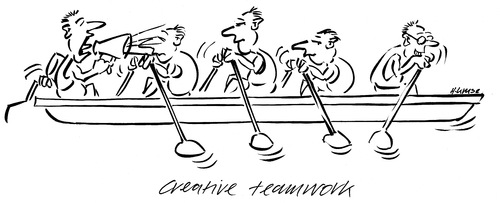
\includegraphics[width=1.00\textwidth]{../../Graphics/creative_teamwork.jpg}
\caption{What's wrong with this picture?}
\end{figure}

\subsection{Open Communication}
A team is able to communicate effectively and there is a feeling of open communication between all members of the group. Issues within a team are handled by face-to-face communication. Team members do not talk behind each other's back as there is a respect developed among team members that necessitates direct and open communication on all issues.

\subsection{Decision-Making}
A team has a hierarchy and a built-in decision-making system that helps it to react quickly and effectively to all situations. The members of the group are respected for their various areas of expertise, and the leader of the group has developed the ability to obtain the group members' opinions to formulate the group's response. This applies to decisions made within the group ranging from resolving internal conflict to a potential change in group leadership.

\subsection{Efficient Use of Ideas}

Brainstorming is one way that groups come up with the solution to a problem. An effective team is able to gather information from each member and formulate that information into a response. The team becomes adept at dismissing ideas that will not work, and including effective ideas into what would become the team's solution to an issue.

\section{Contract}

Each team will develop a contract, based on the contract template available in github/Admin. The language that you choose will vary based on your team, below is a template that you might find useful:

\subsection{Aspirations}

Developing aspariational goals allows the team to evaluate their process at a fairly high level with the possibility of drilling down to see how these map onto various activities and expectations. 

\begin{itemize}
  \item We all promise to listen to each other's ideas with respect.
  \item We all promise to do our work as best as we can.
  \item We all promise to do our work on time.
  \item We all promise to ask for help if we need it.
  \item We all promise to ???.
\end{itemize}

\subsection{Effort Reporting}

Allowing each team member to contribute is a key part of the process. But also, we need to make sure the workload is equitable. To improve the outcome of this process, it's important to document team member effort.

Each team will develop a method to document your contributions to the overall team effort. Team member contributions will contribute to the grade for this project. The format and methods of documenting the contributions must be decided AND developed before the contract is signed.

\subsection{Consequences}

When agreements are broken without consequences, team members can become resentful. To avoid this, we should specify the consequences if the contract rules are broken. Please avoid being punative. Here's an example that you might find useful:

\begin{quote}
If someone on our team breaks one or more of our rules, we will ask why were the rules not followed. As we evaluate the conversation, we will augment the rule or ask the person to follow our agreement. If the person continues to break the rules, we will ask the professor to help find a solution.
\end{quote}

\noindent Please note, individual follow through on the contract agreement will be reflected in the project grade.

\subsection{Signatures}

Finally, your contract shall include a signature page with a line for each team member and instructor (based on expectations you have defined outline).

\end{document}
